\documentclass[12pt]{article}
\usepackage{amsmath}
\usepackage{amssymb} %mathbb
\usepackage{graphicx}
\usepackage{hyperref}
\usepackage{xcolor}
\usepackage{cancel}
\usepackage[latin1]{inputenc}
\usepackage[paperheight=377mm,paperwidth=210mm,top=1.0cm,bottom=1.3cm,left=1.0cm,right=1.0cm,landscape]{geometry}

\begin{document}

\Large

\begin{center}
\textbf{Geometria Convexa | Dualidade | Transformada de Legendre}
\end{center}

\large

V\'ideo Principal no \href{https://www.youtube.com/watch?v=KlShZXH1WrE}{\color{blue}\underline{YouTube}}.

\vspace{3mm}

C\'alculos b\'asicos em uma dimens\~ao. Par\'abolas, elipses, hip\'erboles:

\begin{align}
g(x) &= ax^2 + bx + c \\
\mathcal{L}(g(x)) = h(y) &= \sup \{ \underbrace{yx - ax^2 - bx - c}_{Ax^2 + Bx + C}\,;\,\forall x \in \mathbb{R} \} \\
A &= -a \\
B &= y - b \\
C &= -c \\
\sup &= -\cfrac{\Delta}{4A} = \cfrac{B^2+4aC}{4a} = \cfrac{(y-b)^2}{4a} - c = a'y^2 + b'y + c' = h(y)
\end{align}

\vspace{3mm}

C\'alculos b\'asicos em duas dimens\~oes. Paraboloides, elipsoides, hiperboloides:

\begin{align}
g(x,y) &= \sigma \sqrt{ax^2 + bxy + cy^2 + dx + ey + f} \\
\mathcal{L}(g(x,y)) = h(u,v) &= \sup \{ \underbrace{ux + vy - \sigma \sqrt{ax^2 + bxy + cy^2 + dx + ey + f}}_{\varphi(x,y)}\,;\,\forall x,y \in \mathbb{R} \} \\
\varphi_x &= u - \sigma \cfrac{2ax + by + d}{2\sqrt{ax^2 + bxy + cy^2 + dx + ey + f}} \\
\varphi_y &= v - \sigma \cfrac{bx + 2cy + e}{2\sqrt{ax^2 + bxy + cy^2 + dx + ey + f}}
\end{align}

\vspace{300mm}

Insisto em c\'alculos b\'asicos em duas dimens\~oes. Paraboloides, elipsoides, hiperboloides:

\begin{align}
g(x,y) &= \sigma \sqrt{ax^2 + bxy + cy^2 + dx + ey + f} \\
\mathcal{L}(g(x,y)) = h(u,v) &= \sup \{ \underbrace{ux + vy - \sigma \sqrt{ax^2 + bxy + cy^2 + dx + ey + f}}_{\varphi(x,y)}\,;\,\forall x,y \in \mathbb{R} \} \\
\varphi_x &= u - \sigma \cfrac{2ax + by + d}{2\sqrt{ax^2 + bxy + cy^2 + dx + ey + f}} \\
\varphi_y &= v - \sigma \cfrac{bx + 2cy + e}{2\sqrt{ax^2 + bxy + cy^2 + dx + ey + f}} \\
D^2 \varphi &= \begin{pmatrix} \varphi_{xx} & \varphi_{xy} \\ \varphi_{xy} & \varphi_{yy} \end{pmatrix}\text{ semi positiva definida }\Leftrightarrow \langle [H\varphi]\cdot \vec w, \vec w\rangle \ge 0, \forall \vec w \in \mathbb{R}^2 \\
\nabla \varphi &= (0, 0) \Rightarrow (u,v) = \beta(x,y) \\
4u^2 (ax^2 + bxy + cy^2 + dx + ey + f) &= (2ax + by + d)^2 \\
Ax^2 + Bx + C &= 0 \Rightarrow x = \gamma_1(u, y) \\
A &= 4au^2 - 4a^2 \\
B &= 4bu^2y + 4du^2 - 4a(by + d) \\
C &= 4cu^2y^2 + 4eu^2y + 4fu^2 - (by + d)^2 \\
4v^2 (ax^2 + bxy + cy^2 + dx + ey + f) &= (bx + 2cy + e)^2 \\
Dy^2 + Ey + F &= 0 \Rightarrow y = \gamma_2(v, x) \Rightarrow (x_0,y_0) = (\psi_1(u, v), \psi_2(u, v)) \\
h(u,v) &= \varphi(x_0, y_0) = (\varphi \circ \psi)(u, v)
\end{align}

Vamos agora para $n$ dimens\~oes.

\vspace{300mm}

		\begin{center}
		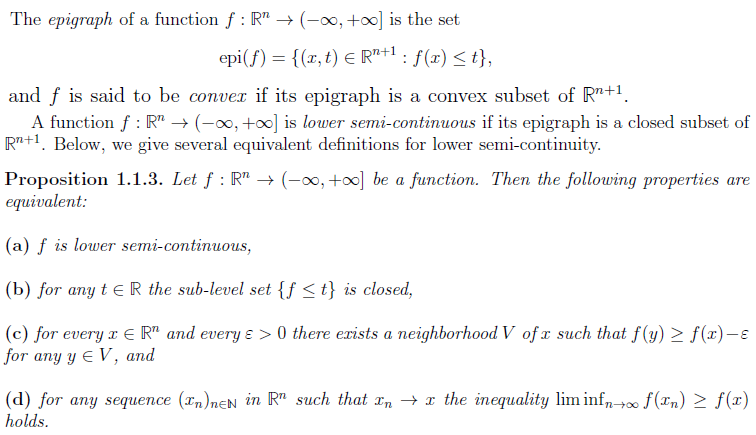
\includegraphics[scale=1.3]{1a}
		\end{center}

0.1. Necess\'ario do in\'icio do livro.

\vspace{300mm}

\vspace{3mm}

		\begin{center}
		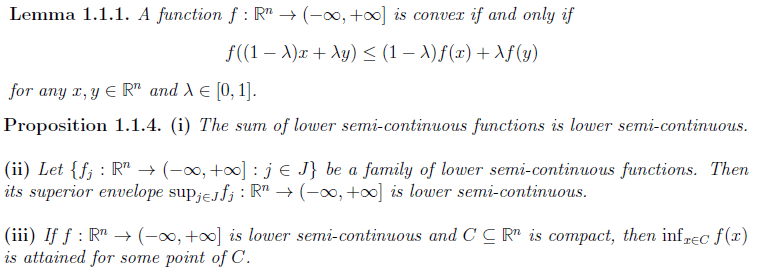
\includegraphics[scale=1.7]{1b}
		\end{center}

0.2. Necess\'ario do in\'icio do livro.

\vspace{300mm}

\vspace{3mm}

		\begin{center}
		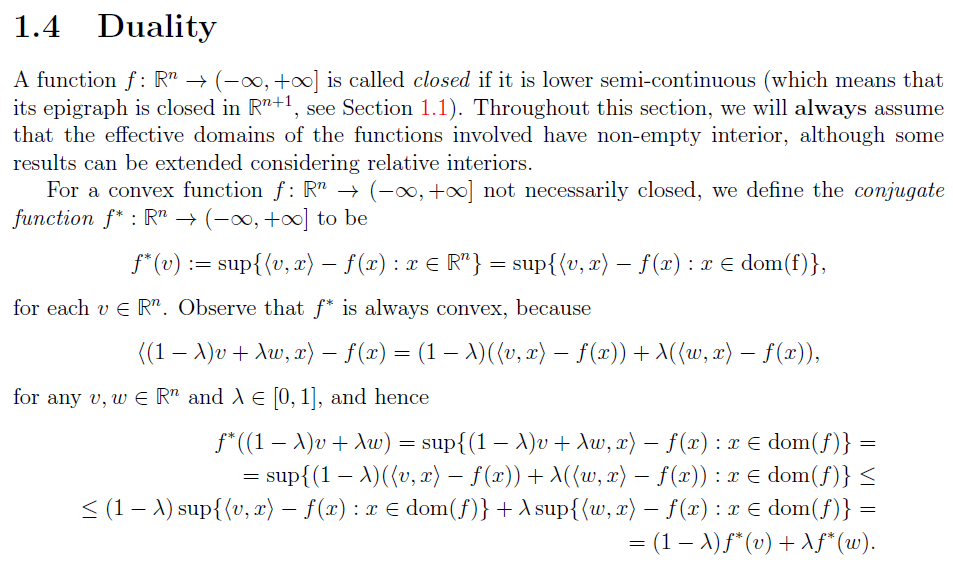
\includegraphics[scale=1.1]{1c}
		\end{center}

1.1. $f^* = \mathcal{L}(f)$. a transformada de Legendre de $f$. Linearidade.

\vspace{300mm}

		\begin{center}
		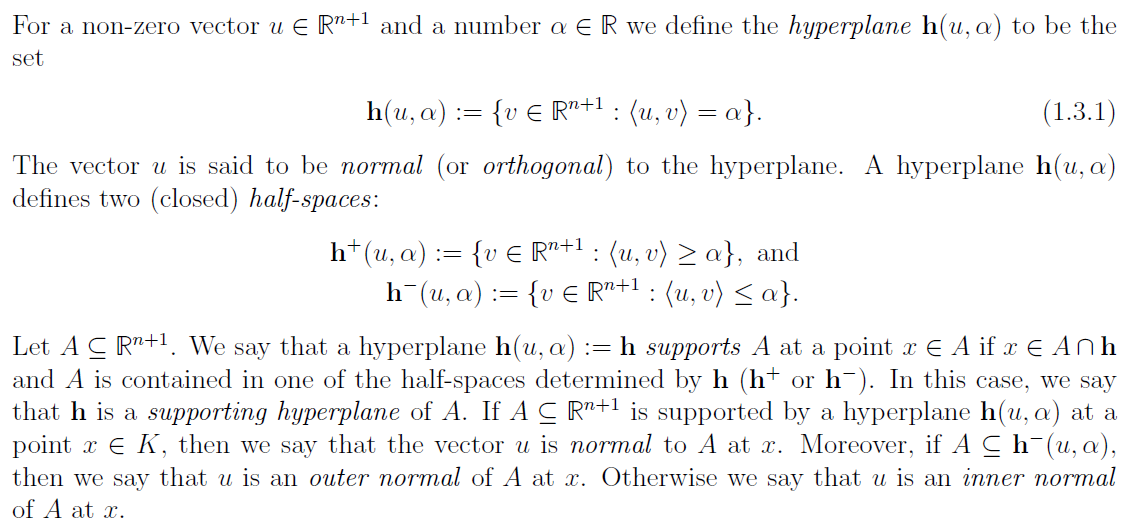
\includegraphics{2a}
		\end{center}

0.3. No plano, por exemplo. $u = (3, 4) \Rightarrow \langle u, (x,y)\rangle \le 11 \Rightarrow 3x + 4y \le 11 \Rightarrow y \le \cfrac{11 - 3x}{4}$.

Seja $x = 1$. Normal para fora. Por defini\c{c}\~ao o normal para dentro \'e o contr\'ario.

\vspace{300mm}

		\begin{center}
		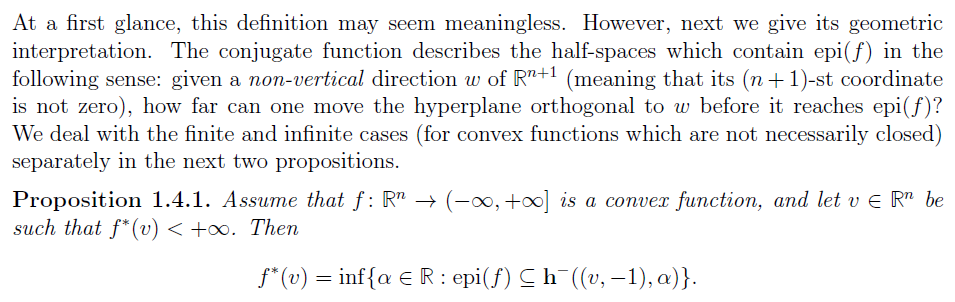
\includegraphics[scale=1.25]{2b}
		\end{center}

Proposi\c{c}\~ao 1.4.1.A. O vertical do autor no plano \'e exatamente o nosso horizontal do mundo real. $y = 0, \forall x\in \mathbb{R}$. A normal \'e que \'e vertical no mundo real.

A partir daqui, fazemos a \'ultima coordenada ser $-1 = y$.

\vspace{300mm}

		\begin{center}
		
\includegraphics{3}
		\end{center}

Proposi\c{c}\~ao 1.4.1.B. $x < x$ \'e absurdo para todo $x$.

\vspace{300mm}

		\begin{center}
		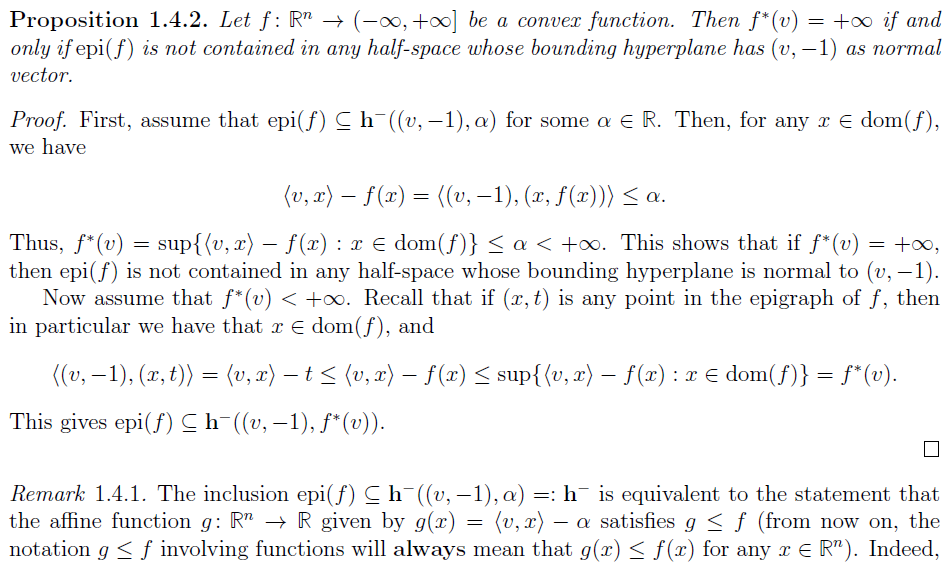
\includegraphics{4}
		\end{center}

Teorema 1.4.2.

Observa\c{c}\~ao 1.4.1.A. Vide fun\c{c}\~ao afim no pr\'oximo slide.

\vspace{300mm}

		\begin{center}
		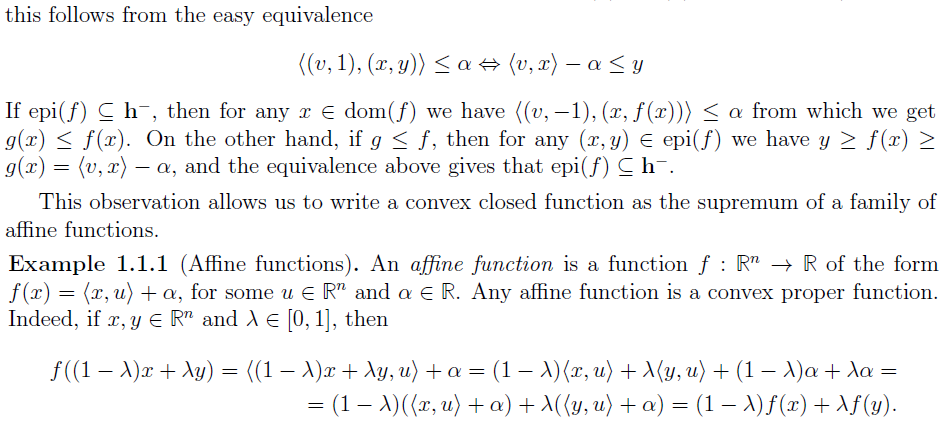
\includegraphics[scale=1.2]{5}
		\end{center}

Observa\c{c}\~ao 1.4.1.B. Uma fun\c{c}\~ao fechada convexa \'e o supremo de v\'arias fun\c{c}\~oes afins. A seguir.

0.4. Necess\'ario do in\'icio do livro.

\vspace{300mm}

		\begin{center}
		
\includegraphics[scale=1.2]{6}
		\end{center}

Teorema 1.4.3.A. A seguir: n\~ao h\'a ponto que pertence a $U$ e n\~ao pertence a epi$(f)$.

\vspace{300mm}

		\begin{center}
		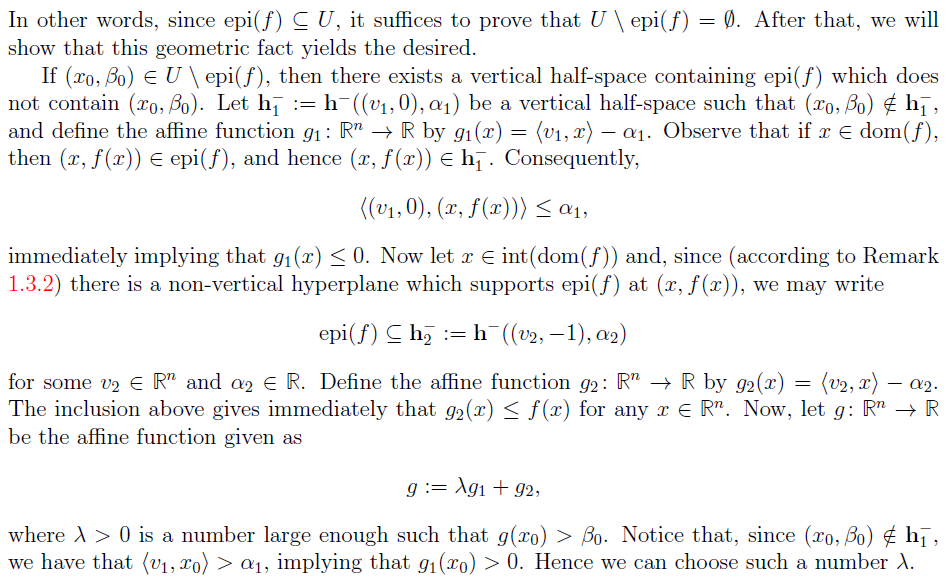
\includegraphics{7a}
		\end{center}

Teorema 1.4.3.B. Vide observa\c{c}\~ao 1.3.2 no pr\'oximo slide.

\vspace{300mm}

		\begin{center}
		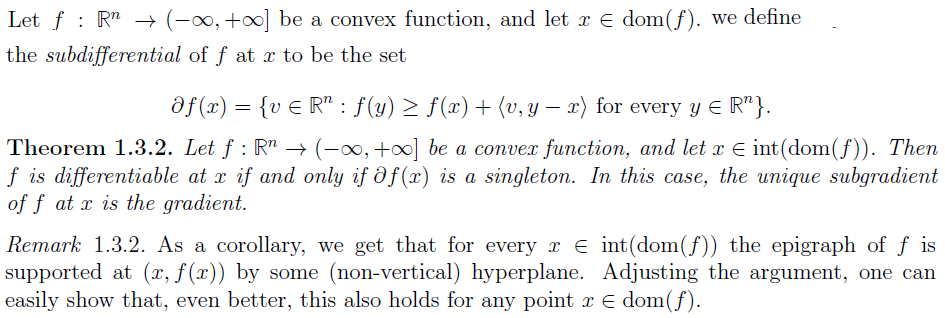
\includegraphics[scale=1.25]{7b}
		\end{center}

0.5. Necess\'ario do in\'icio do livro.

\vspace{300mm}

		\begin{center}
		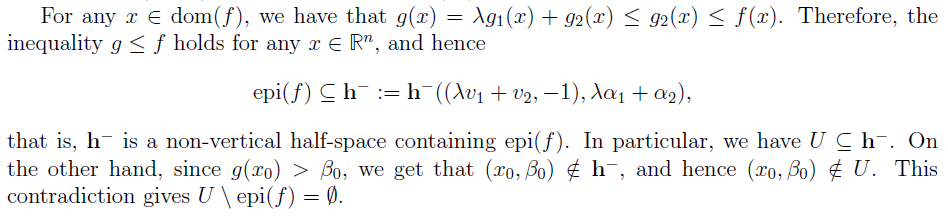
\includegraphics[scale=1.25]{8}
		\end{center}

Teorema 1.4.3.C. Contram\~ao.


\vspace{300mm}

		\begin{center}
		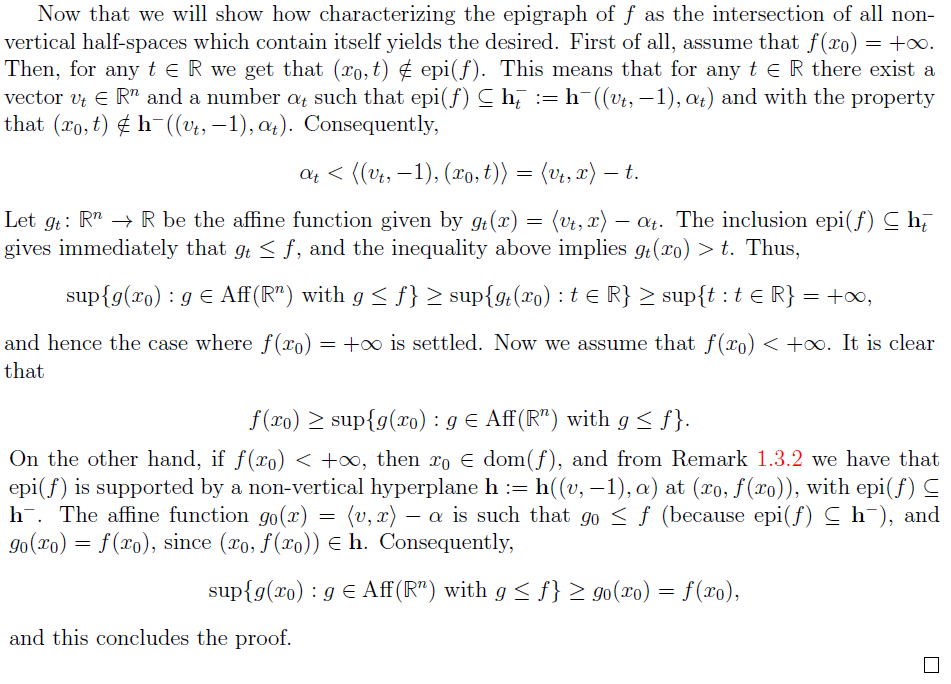
\includegraphics[scale=.9]{9}
		\end{center}

Teorema 1.4.3.D. Usamos que $U = \text{epi}(f)$ para mostrar que $f(x) = \sup \{ g(x) \}$, como quer\'iamos desde o princ\'ipio.

\vspace{300mm}

		\begin{center}
		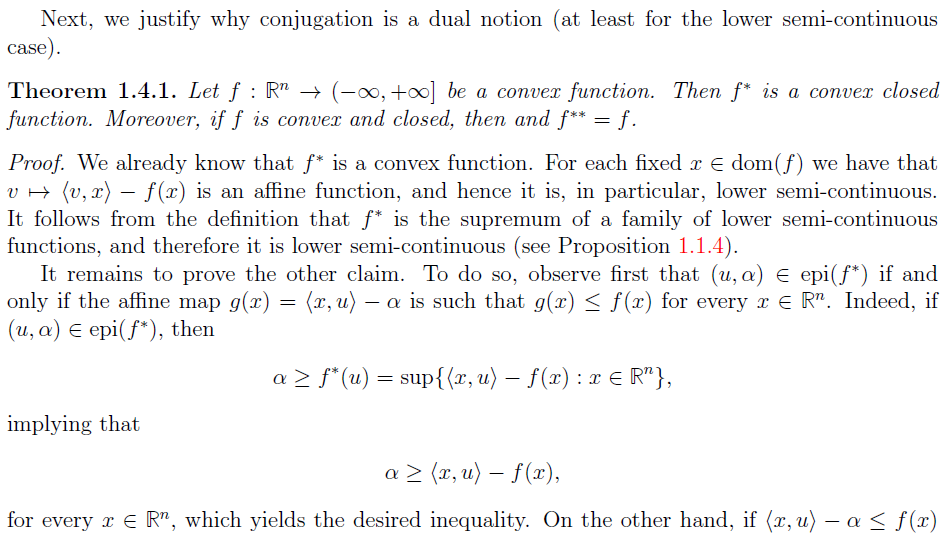
\includegraphics{10}
		\end{center}

Teorema 1.4.1.A. Falta mostrar que $\mathcal{L}(f(x) = f^*(v) \Rightarrow \mathcal{L}(\mathcal{L}(f(x))) = \mathcal{L}(f^*(v)) = f(x)$.

\vspace{300mm}

		\begin{center}
		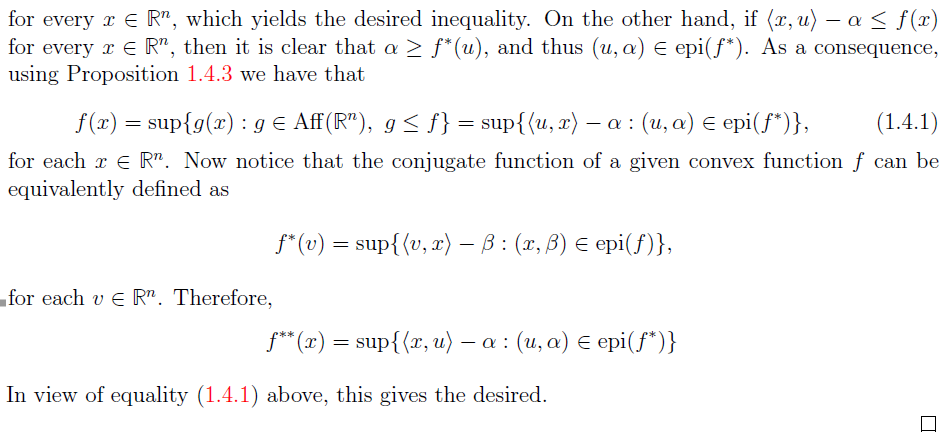
\includegraphics{11}
		\end{center}

Teorema 1.4.1.B.

\vspace{12mm}

\Large

\begin{center}
\textbf{Obrigado}
\end{center}

\large

\vspace{12mm}

Fora da caridade, n\~ao h\'a salva\c{c}\~ao. Com caridade, h\'a evolu\c{c}\~ao.

Vinicius Claudino Ferraz, vers\~ao $0.2.\sigma$ de 17/fev/2020.

\end{document}
